\section{Profondità di campo} \label{sec:dof}
La \textbf{profondità di campo}, in inglese \textit{depth of field}, rappresenta la zona dell'immagine messa a fuoco, ovvero quella con maggiore nitidezza.

\begin{figure}[h]
    \centering
    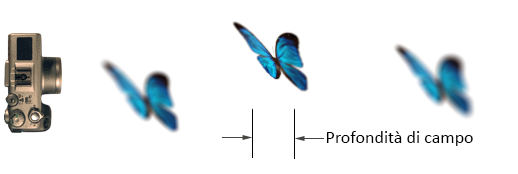
\includegraphics[width=0.9\textwidth]{PdC.png}
\end{figure}

Avere maggiore profondità di campo significa avere una più grande zona a fuoco, mentre restringere la profondità di campo significa avere una porzione dell'inquadratura messa a fuoco più stretta.

Quando la profondità di campo diventa più piccola non solo l'area messa a fuoco diventa più piccola, ma le porzioni che non sono messe a fuoco diventano sempre "più sfocate", meno nitide.

Vediamo un esempio pratico per capire meglio cosa succede: immaginiamo i riprendere una lampaina accesa, se spostiamo la messa a fuocom per mettere a fuoco sempre più vicino a noi, la profondità di campo diminuisce e la lampadina man mano che diventa sfocata si trasforma, nella nostra immagine, in un cerchio di luce sempre più grande e indefinito. In questo senso diventa tutto "più sfocato".

\begin{figure}[h]
    %\centering
    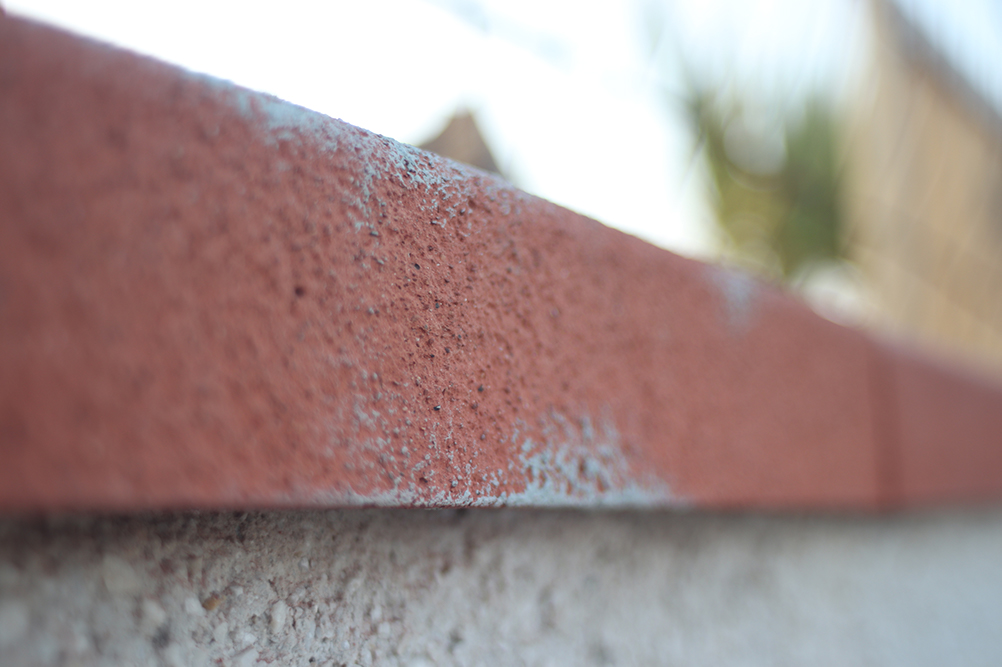
\includegraphics[width=0.88\textwidth]{Muro.jpg}
    \caption{
        In questa foto, scattata a distanza molto ravvicinata dal muretto, si può vedere bene la profondità di campo
    }
\end{figure}

\subsection{Modificare la profondità di campo} \label{subsec:modificadof}
Ad influenzare la profondità di campo sono tre fattori:
\begin{itemize}
    \item[-] Lunghezza focale
    \item[-] Distanza dal soggetto
    \item[-] Diaframma
\end{itemize}

Più aumenta la \textbf{lunghezza focale} minore sarà la profondità di campo, e viceversa.\newline
Un teleobiettivo tende a staccare molto il soggetto dal resto della foto; se si fa un ritratto con un teleobiettivo si otiene una persona bene a fuoco, con lo sfondo completamente sfocato.
Diversamente un grandangolo può aumentare così tanto la profondità di campo da poter avere, senza troppa difficoltà, l'intera inquadratura a fuoco.

Aumentando la \textbf{distanza dal soggetto} aumenta la profondità di campo, e viceversa.\newline
Per distanza dal soggetto si intende cosa mettiamo a fuoco nella foto; se in una foto il nostro soggetto è una persona, allora implicitamente sappiamo che questa persona sarà messa a fuoco.
Prendiamo due estremi per capire meglio: macro e fotografia di montagna. In una foto macro, in cui siamo estremamente vicini al soggetto, la profondità di campo è piccolissima (così tanto che spesso per avere il soggetto completamente a fuoco è necessario fare più scatti mettendo a fuoco ogni volta un pezzo diverso), con lo sfondo talmente sfocato da apparire, spesso, quasi a tinta unita. Se invece fotografiamo una montagna, molto lontana da noi, la profondità di campo aumenta così tanto che tutta la foto è a fuoco.

Aprire il \textbf{diaframma} diminuisce la profondità di campo, mentre chiuderlo la aumenta (vedi \nameref{sec:diaframma}).


\subsection{Distanza iperfocale} \label{subsec:iperfocale}
La distanza iperfocale è la distanza alla quale bisogna mettere a fuoco per avere tutta l'inquadratura a fuoco.

Come sapere la distanza alla quale stiamo mettendo a fuoco? Alcuni obiettivi hanno una ghiera o delle tacchette incorporate che danno questa informazione, se l'obiettivo non ci aiuta si può andare ad occhio.

La distanza iperfocale ovviamente non è fissa, e dipende dalla focale della nostra lente, dall'apertura e dalla grandezza del sensore.

Online si trovano moltissime tabelle che ci dicono le distanze iperfocali, già calcolate, per diverse combinazioni di lenti, aperture e sensori. All'occorrenza possiamo calcolare l'iperfocale con una semplice formula:
\[ H = \dfrac{f^2}{N \cdot c} + f \]
Dove:
\begin{itemize}
    \item[-] $H$ è la distanza iperfocale, espressa in millimetri
    \item[-] $f$ è la lunghezza focale
    \item[-] $N$ è l'apertura del diaframma
    \item[-] $c$ è il circolo di confusione\footnote{
        Nota dell'autore: il circolo di confusione è un concetto fisico che non solo non conosco, ma che è in ogni caso fuori dallo \textit{scope} di questo manuale, mi limiterò quindi a fornire qualche valore notevole da poter usare per calcolare l'iperfocale
    }, espresso in millimetri
\end{itemize}

\nb Il valore della lunghezza focale è talmente piccolo rispetto al valore della frazione che si può omettere nella formula, ovvero è sufficiente fare la frazione senza poi sommare la focale (i.e. $+ f$).

I valori del circolo di confusione sono noti, e si trovano facilmente in rete molte tabelle.
A seguire sono riportati alcuni valori di interesse del circolo su diversi sensori:
\begin{itemize}
    \item[-] APS-C Canon: $0.018$mm
    \item[-] APS-C Nikon: $0.019$mm
    \item[-] Full frame: $0.029$mm
\end{itemize}